\section{Diseño de PCB}
EL objetivo de esta estapa es diseñar un filtro pasa-banda cuya banda pasante sea las frecuencias de la voz humana. Según la investigación realizada dicha banda va desde los $300Hz$ hasta $3400Hz$. Para ello se tuvo en cuenta la combinación de un filtro pasa-altos y un filtro pasa-bajos unidos por un amplificador operacional(en este caso un TL072 pues es el que mejores resultados ha dado). El amplificador no inversor sirve para que la primera etapa no cargue a la segunda y el buffer se utilza para evitar que el circuito que se le pone a la salida cargue el filtro. Todo esto es posbile gracias a la alta impedancia de entrada del amplificador operacional. El filtro sigue la configuración del siguiente esquemático:

\begin{figure}[H]
    \centering
    \begin{tikzpicture}[scale=0.75, transform shape]
    	% Paths, nodes and wires:
    	\node[shape=rectangle, minimum width=-0.035cm, minimum height=-0.035cm] at (0, -0){};
    	\node[shape=rectangle, minimum width=-0.035cm, minimum height=-0.035cm] at (0, -0){};
    	\draw (-30, -0) to[capacitor, l={$C_{Pa}$}] (-26.663, 0.006);
    	\draw (-20.917, 0.467) to[capacitor, l={$R_{Pb}$}] (-20.867, -3.045);
    	\draw (-26.663, 0.006) to[american resistor, l={$R_{Pa}$}] (-26.663, -3.121);
    	\draw (-20.917, 0.467) to[american resistor, l={$R_{Pb}$}] (-23.854, 0.489);
    	\node[op amp] at (-25.044, 0.489){};
    	\draw (-26.663, 0.006) -| (-26.234, -0.001);
    	\draw (-26.234, 2.462) to[american resistor, l={$R_{out}$}] (-23.718, 2.501);
    	\draw (-26.698, 2.462) to[american resistor, l={$R_{in}$}] (-26.698, 4.577);
    	\draw (-26.698, 0.99) |- (-26.234, 2.462);
    	\draw (-23.718, 2.501) |- (-23.854, 0.489);
    	\node[op amp] at (-18.82, 0.957){};
    	\draw (-20.917, 0.467) -| (-20.01, 0.505);
    	\draw (-20.01, 1.447) -| (-20.716, 1.447) |- (-20.698, 2.64) -| (-17.63, 0.957);
    	\draw (-17.63, 0.957) -| (-15.965, 1.003);
    	\node[ground] at (-26.663, -3.121){};
    	\node[ground] at (-20.867, -3.045){};
    	\node[ground, xscale=-1, yscale=-1] at (-26.698, 4.577){};
    	\draw (-25.83, 0.966) -| (-26.698, 0.99);
    	\draw[-latex] (-29.357, -3.389) -- (-29.349, -0.338);
    	\draw[-latex] (-16.691, -2.98) -- (-16.683, 0.072);
    	\node[shape=rectangle, minimum width=1.282cm, minimum height=1.131cm](N1) at (-30.152, -1.828){} node[anchor=center] at (N1.text){$V_{in}$} node[anchor=north west, align=left, text width=0.894cm, inner sep=6pt] at (-30.81, -1.245){};
    	\node[shape=rectangle, minimum width=1.337cm, minimum height=1.159cm](N2) at (-15.977, -1.389){} node[anchor=center] at (N2.text){$V_{out}$} node[anchor=north west, align=left, text width=0.949cm, inner sep=6pt] at (-16.663, -0.792){};
    \end{tikzpicture}
    \caption{Esquemático del filtro}
    \label{fig:filtro_PAPB}
\end{figure}

Los componentes utilizados en para el diseño de dicho filtro son:

\begin{table}[H]
    \centering
    \label{tab:mi_tabla}
    \begin{tabular}{|c|c|c|}
        \hline
        Resistencia & Nominal & Medido\\
        \hline
        $R_{Pa}[k\Omega]$ & $1.5$ & $1.465$ \\
        \hline
        $R_{Pb}[k\Omega]$ & $0.82$ & $0.82$ \\
        \hline
        $R_{in}[k\Omega]$ & $5.6$ & $5.5$\\
        \hline
        $R_{out}[k\Omega]$ & 1 & $0.985$ \\
        \hline
        Capacitores & Nominal & -\\
        \hline
        $C_{Pa}[nF]$ & $220$ &-\\
        \hline
        $C_{Pb}[nF]$ & $68$ & -\\
        \hline
    \end{tabular}
    
        \caption{Componentes del filtro pasa banda}
    \label{tab:Comp_filtro}
\end{table}

La función transferencia del filtro es:

\begin{equation}
H(s) = R_{Pa} C_{Pa} G
\frac{s}
{(s R_{Pa} C_{Pa} + 1)(s R_{Pb} C_{Pb} + 1)}
\end{equation}

Siendo G la ganancia del amplificador operacional dada por la ecuación \ref{eq_Gan}.

\begin{equation}
    G = 1 + \frac{R_{out}}{R_{in}}
    \label{eq_Gan}
\end{equation}

 El diagrama de polos y ceros del diseño:

\begin{figure}[H]
    \centering
    \usetikzlibrary{shapes.geometric}
    \begin{tikzpicture}[scale = 1.5, transform shape]
    	% Paths, nodes and wires:
    	\node[shape=rectangle, minimum width=-0.035cm, minimum height=-0.035cm] at (0, -0){};
    	\node[shape=rectangle, minimum width=-0.035cm, minimum height=-0.035cm] at (0, -0){};
    	\draw[-latex] (-25, -5) -- (-25, -0);
    	\draw[-latex] (-28.43, -2.262) -- (-21.664, -2.279);
    	\node[shape=rectangle, minimum width=0.531cm, minimum height=0.219cm](N1) at (-24.223, -0.093){} node[anchor=center] at (N1.text){$j\omega$} node[anchor=north west, align=left, text width=0.143cm, inner sep=6pt] at (-24.506, 0.034){};
    	\node[shape=rectangle, minimum width=0.298cm, minimum height=0.502cm](N2) at (-21.83, -2.01){} node[anchor=center] at (N2.text){$\sigma$} node[anchor=north west, align=left, text width=-0.09cm, inner sep=6pt] at (-21.997, -1.741){};
    	\node[shape=rectangle, minimum width=0.505cm, minimum height=0.485cm](N3) at (-23.033, -0.275){} node[anchor=center] at (N3.text){$S)$} node[anchor=north west, align=left, text width=0.117cm, inner sep=6pt] at (-23.303, -0.015){};
    	\node[shape=ellipse, draw={rgb,255:red,160;green,84;blue,158}, line width=1pt, minimum width=0.135cm, minimum height=0.137cm] at (-24.999, -2.272){};
    	\path[draw={rgb,255:red,60;green,236;blue,183}] (-26.052, -2.395) -- (-25.642, -2.126);
    	\path[draw={rgb,255:red,60;green,236;blue,183}] (-25.661, -2.446) -- (-26.042, -2.097);
    	\node[shape=rectangle, minimum width=0.542cm, minimum height=0.564cm](N4) at (-25.95, -2.746){} node[anchor=center] at (N4.text){$-3030$} node[anchor=north west, align=left, text width=0.154cm, inner sep=6pt] at (-26.238, -2.446){};
    	\path[draw={rgb,255:red,60;green,236;blue,183}] (-28.191, -2.386) -- (-27.781, -2.117);
    	\path[draw={rgb,255:red,60;green,236;blue,183}] (-27.8, -2.437) -- (-28.181, -2.088);
    	\node[shape=rectangle, minimum width=1.255cm, minimum height=0.419cm](N5) at (-28.134, -2.83){} node[anchor=center] at (N5.text){$-18000$} node[anchor=north west, align=left, text width=0.867cm, inner sep=6pt] at (-28.779, -2.603){};
    \end{tikzpicture}
    \caption{Gráfico de polos y ceros}
    \label{fig:pol_cer}
\end{figure}

El presente filtro es un fitro de primer orden en dos etapas. La primera etapa es un filtro pasa-altos cuya frecuencia de corte es $\omega_l=\frac{1}{R_{Pa} \cdot C_{Pa}} \sim 3030 rad/s$. En la segunda etapa se presenta un filtro pasa-bajos cuya frecuencia de corte es $\omega_h = \frac{1}{R_{Pb} \cdot C_{P_b}} \sim 18000 rad/s$. La ventaja que posee trabajar con etapas de primer orden es la sencillez y una desviación del modelo ideal muy inferior a comparación de trabjar con un segundo orden. La desventaja en este caso es que por más de que se adecuen acordemente las frecuencias de corte, la atenuación que presenta por fuera de la banda pasante crece de manera lenta. Se observa una pendiente de aproximadamente $-20\frac{dB}{dec}$ mientras que con un filtro de segundo orden la pendiente con la cual decrece la transferencia sería el doble, produciendo así un mejor filtrado de la frecuencia deseada. Además, fue necesario introducir una ganancia al diseño para subir la curva y terminar de acomodar las frecuencias que delimitan la banda pasante. Estas frecuencias se llamarán $f_{c1}$ para la frecuencia inferior y $f_{c2}$ para la superior. Ambas son las frecuencias que se encuentran sobre la línea de $-3dB$. 

Se eligieron resistencias altas para así poder despreciar la resistencia que le pueda cargar el generador al filtro. A su vez, los valores de resistencia y capacitor se seleccionaron de forma tal que las frecuencias de corte de la banda resultaran cercanas a las frecuencias de corte deseadas tomando en cuenta que la banda pasante se consideraría la banda que se eencuentra atenuada menos de $-3dB$. Posteriormente, se probó el filtro en el laboratorio y se ajustaron los valores de las resistencias para que quede la banda lo más cercano a $300Hz$ y $3400Hz$. 
Todo esto se probó con dos buffers en vez de un buffer y un operacional con ganancia. Una vez ajustadas las frecuencias de corte, se calculó la ganancia que debería introducirse para que la banda se encontrara sobre el eje de las abscisas con la  fórmula \ref{eq_Gan}. G (la ganancia) en este caso sería cuánto se debería subir la gráfica. Tomando $R_{out} = 1k\Omega$ se puede despejas $R_{in}$. En este sentido, la ganancia sería 1.20.

En la siguiente figura se puede observar la curva de la que se ha estado hablando en esta sección. 


\begin{figure}[H]
    \centering
    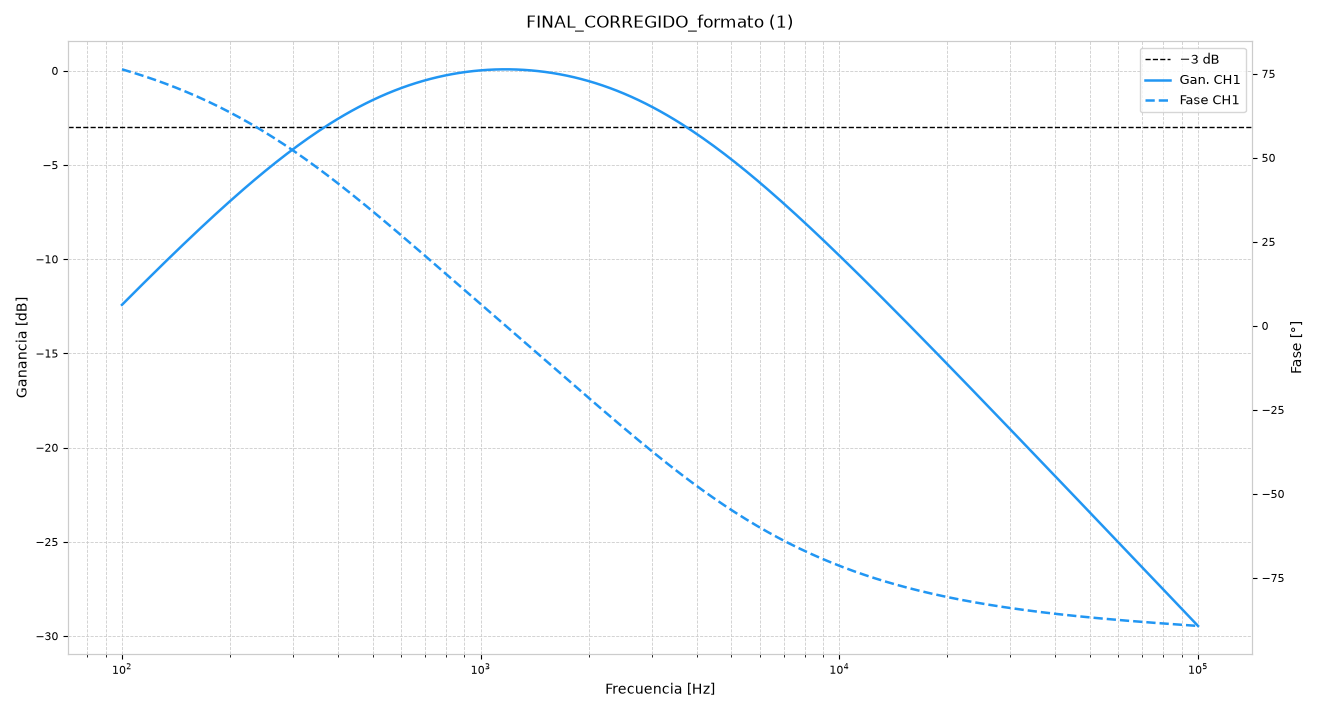
\includegraphics[width=1\textwidth]{BODE_REAL_FILTRO.png}
    \caption{respuesta medida del filtro }
    \label{fig:Bode_filtro_real}
\end{figure}

\begin{figure}[H]
    \centering
    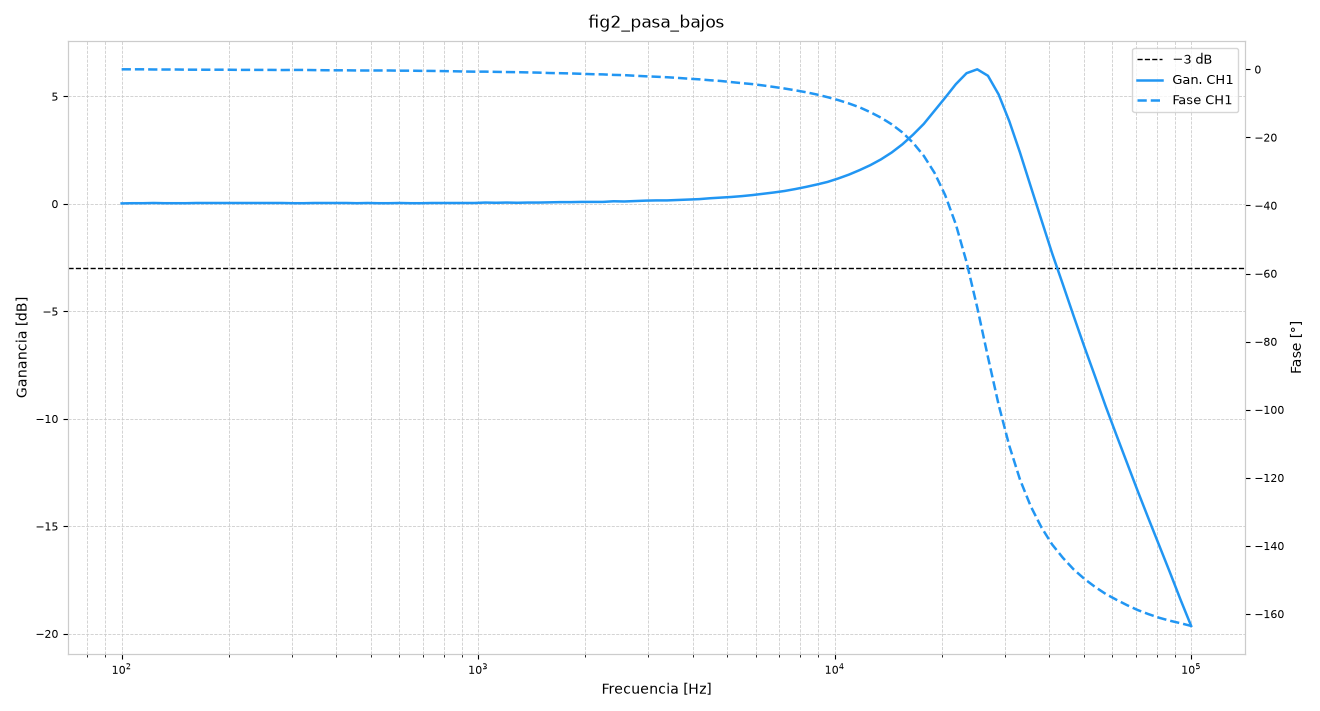
\includegraphics[width=1\textwidth]{BODE_SIMULADO_FILTRO.png}
    \caption{respuesta simulada del filtro }
    \label{fig:Bode_filtro_sim}
\end{figure}

No se observan discrepancias importantes entre ambas gráficas. Las diferencias podrían explicarse por la tolerancia del capacitor.  

\subsection{Análisis del Filtro}
En la figura \ref{fig:Bode_filtro_real} y \ref{fig:Bode_filtro_sim} se observa que la frecuencia $f_{c2}$ se encuentra lo suficientemente cercana a  $3400Hz$. En los graves, se observa que la banda está  $60Hz$ más alta de lo deseado. Sin embargo es una diferencia de un $3\%$ del ancho de banda total. En consecuencia, no tendrá un gran impacto en la calidad de filtrado.
El único problema que se percibe y es irreconciliable por el mismo diseño del filtro es que no tienen cortes limpios. En otras palabras, no sucede que solo la banda pasante es la que no se atenúa. Al tener una pendiete tan pequeña, comparado con lo que se podría lograr con un filtro de segundo orden en dos etapas, las frecuencias que no pertenecen a la banda pasante todavía podrían ser percibidas con una atenuación pequeña. Esta sería una caracterítica a mejorar pero igualmente se podria distingir la banda pasante por sobre las demás frecuencias así que cumple con su propósito de filtro en un nivel muy básico. 
Una posible mejora que no se ha tenido en cuenta en este diseño es la utilización de capacitores de desacople para la alimentación del TL072. Estos capacitores se conectarían como indica la figura \ref{fig:C_des} y sirven para mantener estable la señal a la que están conectadas. Es una buena práctica utilizarlas. 

\begin{figure}[H]
    \centering
    \begin{tikzpicture}[transform shape]
    	% Paths, nodes and wires:
    	\node[op amp] at (-22.458, -7.516){};
    	\draw (-22.541, -6.977) to[capacitor, l={$C_{desacople}$}] (-22.559, -4.406);
    	\draw (-22.541, -8.055) to[capacitor, l={$C_{desacople}$}] (-22.546, -10.709);
    	\node[shape=rectangle, minimum width=1.424cm, minimum height=0.581cm] at (-22.559, -4.098){} node[anchor=north west, align=left, text width=1.036cm, inner sep=6pt] at (-23.289, -3.789){+15V\\};
    	\node[shape=rectangle, minimum width=1.424cm, minimum height=0.581cm] at (-22.546, -11.018){} node[anchor=north west, align=left, text width=1.036cm, inner sep=6pt] at (-23.276, -10.709){-15V\\};
    \end{tikzpicture}
    \caption{Esquemático para la conexión de capacitores de desacople}
    \label{fig:C_des}
\end{figure}